% Algebraic coordinates (x,u,T) fail at x=0; (y,v,T) fail at y=0.
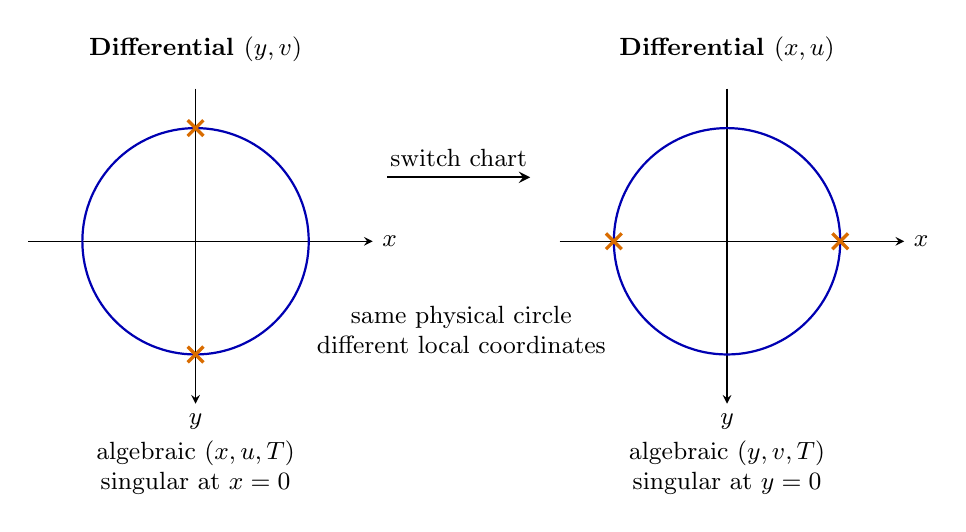
\begin{tikzpicture}[>=stealth,scale=1.25]
\foreach \s/\title in {0/{Differential $(y,v)$},5.4/{Differential $(x,u)$}}{
\begin{scope}[xshift=\s cm]
\node[font=\small\bfseries]at(0,1.95){\title};
\draw[->,black](-1.7,0)--(1.8,0)node[right,font=\small]{$x$};
\draw[->,black](0,1.55)--(0,-1.65)node[below,font=\small]{$y$};
\draw[blue!70!black,thick](0,0)circle(1.15);
\end{scope}}
\foreach \y in {-1.15,1.15}{\draw[orange!85!black,very thick](-.08,\y-.08)--(.08,\y+.08);\draw[orange!85!black,very thick](-.08,\y+.08)--(.08,\y-.08);}
\foreach \x in {4.25,6.55}{\draw[orange!85!black,very thick](\x-.08,-.08)--(\x+.08,.08);\draw[orange!85!black,very thick](\x-.08,.08)--(\x+.08,-.08);}
\node[font=\small,align=center]at(0,-2.3){algebraic $(x,u,T)$\\singular at $x=0$};
\node[font=\small,align=center]at(5.4,-2.3){algebraic $(y,v,T)$\\singular at $y=0$};
\draw[->,thick](1.95,.65)--node[above,font=\small]{switch chart}(3.4,.65);
\node[font=\small,align=center]at(2.7,-.9){same physical circle\\different local coordinates};
\end{tikzpicture}
